%%%%%%%%%%%%%%%%%%%%%%%%%%%%%%%%%%%%%%%%%%%%%%%%%%%%%%%%%%%%%%%%%%%%%%%%%%%%
% AGUJournalTemplate.tex: this template file is for articles formatted with LaTeX
%
% This file includes commands and instructions
% given in the order necessary to produce a final output that will
% satisfy AGU requirements, including customized APA reference formatting.
%
% You may copy this file and give it your
% article name, and enter your text.
%
%
% Step 1: Set the \documentclass
%
%

%% To submit your paper:
\documentclass[draft]{agujournal2019}
\usepackage{url} %this package should fix any errors with URLs in refs.
\usepackage{lineno}
\usepackage[inline]{trackchanges} %for better track changes. finalnew option will compile document with changes incorporated.
\usepackage{soul}
\linenumbers
\usepackage{amsmath} 
\usepackage{gensymb}
%%%%%%%
% As of 2018 we recommend use of the TrackChanges package to mark revisions.
% The trackchanges package adds five new LaTeX commands:
%
%  \note[editor]{The note}
%  \annote[editor]{Text to annotate}{The note}
%  \add[editor]{Text to add}
%  \remove[editor]{Text to remove}
%  \change[editor]{Text to remove}{Text to add}
%
% complete documentation is here: http://trackchanges.sourceforge.net/
%%%%%%%

\draftfalse

%% Enter journal name below.
%% Choose from this list of Journals:
%
% JGR: Atmospheres
% JGR: Biogeosciences
% JGR: Earth Surface
% JGR: Oceans
% JGR: Planets
% JGR: Solid Earth
% JGR: Space Physics
% Global Biogeochemical Cycles
% Geophysical Research Letters
% Paleoceanography and Paleoclimatology
% Radio Science
% Reviews of Geophysics
% Tectonics
% Space Weather
% Water Resources Research
% Geochemistry, Geophysics, Geosystems
% Journal of Advances in Modeling Earth Systems (JAMES)
% Earth's Future
% Earth and Space Science
% Geohealth
%
% ie, \journalname{Water Resources Research}

\journalname{Enter journal name here}


\begin{document}

%% ------------------------------------------------------------------------ %%
%  Title
%
% (A title should be specific, informative, and brief. Use
% abbreviations only if they are defined in the abstract. Titles that
% start with general keywords then specific terms are optimized in
% searches)
%
%% ------------------------------------------------------------------------ %%

% Example: \title{This is a test title}

%\title{An artificial intelligence and budget closure based evaporation correction model at the global scale}
\title{Learning global evapotranspiration dataset corrections from a water cycle closure supervision}

%% ------------------------------------------------------------------------ %%
%
%  AUTHORS AND AFFILIATIONS
%
%% ------------------------------------------------------------------------ %%

% Authors are individuals who have significantly contributed to the
% research and preparation of the article. Group authors are allowed, if
% each author in the group is separately identified in an appendix.)

% List authors by first name or initial followed by last name and
% separated by commas. Use \affil{} to number affiliations, and
% \thanks{} for author notes.
% Additional author notes should be indicated with \thanks{} (for
% example, for current addresses).

% Example: \authors{A. B. Author\affil{1}\thanks{Current address, Antartica}, B. C. Author\affil{2,3}, and D. E.
% Author\affil{3,4}\thanks{Also funded by Monsanto.}}

\authors{Tristan Hascoet\affil{1}, Victor Pellet\affil{2}, and Filipe Aires\affil{2}}

\affiliation{1}{Japon}
\affiliation{2}{France}
% \affiliation{3}{Third Affiliation}
% \affiliation{4}{Fourth Affiliation}

%\affiliation{1}{Kobe address}
%(repeat as many times as is necessary)

%% Corresponding Author:

% (include name and email addresses of the corresponding author.  More
% than one corresponding author is allowed in this LaTeX file and for
% publication; but only one corresponding author is allowed in our
% editorial system.)

% Example: \correspondingauthor{First and Last Name}{email@address.edu}

\correspondingauthor{Tristan Hascoet}{tristan@people.kobe-u.ac.jp}

%% Keypoints, final entry on title page.

%  List up to three key points (at least one is required)
%  Key Points summarize the main points and conclusions of the article
%  Each must be 140 characters or fewer with no special characters or punctuation and must be complete sentences

% Example:
% \begin{keypoints}
% \item	List up to three key points (at least one is required)
% \item	Key Points summarize the main points and conclusions of the article
% \item	Each must be 140 characters or fewer with no special characters or punctuation and must be complete sentences
% \end{keypoints}

\begin{keypoints}
\item Current evapotranspiration (ET) datasets have errors that do not allow to close the global water cycle.
\item Optimal Interpolation (OI) allows to correct catchment-level ET estimates. 
\item We porpose to use Machine Learning to generalize sparse catchment-level ET corrections derived by OI to dense global corrections at the pixel level.
\item Results show our learned pixel-level corrections to reduce water cycle closure errors on held-out test sets for four distinct global ET datasets.
\end{keypoints}

%% ------------------------------------------------------------------------ %%
%
%  ABSTRACT and PLAIN LANGUAGE SUMMARY
%
% A good Abstract will begin with a short description of the problem
% being addressed, briefly describe the new data or analyses, then
% briefly states the main conclusion(s) and how they are supported and
% uncertainties.

% The Plain Language Summary should be written for a broad audience,
% including journalists and the science-interested public, that will not have 
% a background in your field.
%
% A Plain Language Summary is required in GRL, JGR: Planets, JGR: Biogeosciences,
% JGR: Oceans, G-Cubed, Reviews of Geophysics, and JAMES.
% see http://sharingscience.agu.org/creating-plain-language-summary/)
%
%% ------------------------------------------------------------------------ %%

%% \begin{abstract} starts the second page

\begin{abstract}

Evapotranspiration (ET) is one of the most uncertain components of the global water cycle.
Improving global ET estimates is needed to better our understanding 
of the global water cycle so as to forecast the consequences of climate change 
on the future of global water resource distribution.
This work presents a methodology to derive monthly corrections of global ET datasets at 0.25 degree resolution. 
We use ML to generalize sparse catchment-level water cycle closure residual information to global and dense pixel-level residuals. 
Our model takes a probabilistic view on ET datasets and their correction that we use to 
regress catchment-level residuals using a sum-aggregated supervision. 
Using four global ET datasets, we show that our learned model has learned 
ET corrections that accurately generalize its water cycle-closure results to unseen catchments.
\end{abstract}

\section*{Plain Language Summary}


Evapotranspiration (ET) is one of the most uncertain components of the global water cycle.
Improving global ET estimates is needed to better our understanding 
of the global water cycle so as to forecast the consequences of climate change 
on the future of global water resource distribution.
This work presents a methodology to derive monthly corrections of global ET datasets at 0.25 degree resolution. 
We use ML to generalize sparse catchment-level water cycle closure residual information to global and dense pixel-level residuals. 
Our model takes a probabilistic view on ET datasets and their correction that we use to 
regress catchment-level residuals using a sum-aggregated supervision. 
Using four global ET datasets, we show that our learned model has learned 
ET corrections that accurately generalize its water cycle-closure results to unseen catchments.


%% ------------------------------------------------------------------------ %%
%
%  TEXT
%
%% ------------------------------------------------------------------------ %%

%%%%%%%%%%%%%%%%%%%%%%%%%%%%%%%%%%%%%%%%%%%%%
\section{Introduction}
%%%%%%%%%%%%%%%%%%%%%%%%%%%%%%%%%%%%%%%%%%%%%
%Datasets et reference pour evap. Principes. Pas evidents, c'est du modele beaucoup. Des erreurs sont inevitables. Il y a quelques données in situ d'Evaporation (flux towers, REF) mais ce n'est pas suffisant et on a une réelle difficulté a valider et calibrer les datasets acutelles.

Evapotranspiration (ET) is a physical process involving soil and plants in their surrounding weather conditions that is of importance for the terrestrial climate system. 
It links the water, energy, and carbon cycles \cite{Fisher2017} in providing moisture and heat to the atmosphere. 
ET can be decomposed into different components : transpiration, interception loss, bare soil evaporation, snow sublimation, and open water evaporation.

Evapotranspiration is hard to measure. 
The most accurate method is based on the local measurements of vertical turbulent fluxes using {\it in situ} eddy covariance \cite{falge2016}. 
From these turbulent fluxes, the sensible and latent heat are derived and the latter is translated into ET using the latent heat of vaporization for water. 
Unfortunately these {\it in situ} data are really sparse on the Globe, as stressed by global dataset such as FLUXNET \cite{falge2016}, 
and often have limited spatial representativeness, particularly over heterogeneous landscapes \cite{Miralles2011}.

Over the last decade, global ET estimate have been available from satellite observations. 
Although the term "satellite" is commonly used for these products, ET processes are not directly sensed from satellites: 
ET estimates are derived from handcrafted equations relying on specific assumptions and parameterizations. 
The Penman-Monteith equation \cite{Penman1948a, Monteith1965a} is considered the standard model. 
This equation gives a "reference" evapotranspiration, 
based on a radiation term related to temperature and an aerodynamic term related to the vapor pressure deficit and wind speed (Shuttleworth, 2012). 
This reference ET is then modulated by crop and soil specific coefficients such as the stress factor \cite{Penman1948a, Monteith1965a}. 
Due to the frequent unavailability of weather variables needed for its calculations, 
many crop models move toward empirical approaches such as \cite{PRIESTLEY1972} (PT) 
that simplifies the PM equation to calculate reference evapotranspiration. 
Satellite-based ET products have improved our understanding of ET processes worldwide, 
allowing us to understand hydrological processes from local to large spatial scales and at multiple temporal scales \cite{Fassoni-Andrade2021}. 

Current global datasets suffer from 
(i) systematic errors in semiarid regimes and tropical forests, 
(ii) imperfect representations of water stress and canopy interception, and 
(iii) a poorly constrained partitioning of terrestrial evaporation into  \cite{Dorigo2021} XXX. 
ET estimates are bounded by their underlying model that consider precipitation only source of moisture and omit lateral input from floodplain as well as irrigation-based ET \cite{VanDijk2018}. Because of a lack of spatially continuous ground-based measurements of ET, satellite-based products are difficult to validate at large spatial scales.

%De plus en plus d'observation sur le cycle de l'eau. Grace a la fermeture du cycle de l'eau, on a montrer que l'OI permettait d'estimer une variable manquante à partir des autres, ou bien d'optimiser chacune des composantes en fonction de leurs caracteristiques d'incertitudes. On peut donc utiliser ce type d'approche pour optimiser l'evaporation à partir des observations indirectes des autres composantes. Par contre, cela ne peut etre fait qu'a l'echelle du basins, et uniquement sur les bassins sur lesquelles ont a des mesures in situ de river discharge. Donc c'est trop limité.

One of the most common approaches to evaluate global ET estimates has been to measure their consistency with independent estimates of ET based on a terrestrial Water Budget (WB) equation \cite{Rodell2011a,Carter2018}. 
Due to the water mass conservation over a river basin, ET is linked to precipitation $P$, total water storage change $dS$ and river discharge $R$. 
At basin scale scale:
\begin{equation}
    dS-P-R-ET=0.
\end{equation}

It has been shown in the literature that the Optimal Interpolation (OI) framework relying on the WB closure as a constrain for optimisation allowed to 
(i) readjust each of the water components according to their uncertainty \cite{Sahoo2011,Pan2012,Rodell2015a,Aires2014, Pellet2019a} and so that the WB is balanced 
(ii) estimate a missing variable from the others \cite{Munier2014c,Pellet2020,Pellet2021c}. 
This framework allows to evaluate consistent fluxes and storage terms for a balanced WB at global \cite{Rodell2015a} scale for monthly estimates.
%This 
Unfortunately, the OI framework is limited to the basin scale, and has only been successfully applied to basins for which {\it in situ} measurements of river discharge are available. 
There is a need for generalizing these estimates from sparse basin-level estimates to dense pixel-level estimates. 

On way to bridge the local and basin scale is the use of globally available environment variable to characterize the ET regime and correct it accordingly. 
One such tentative was introduced in \cite{Munier2017} where each pixel was characterised based on environmental variables and a quasi linear correction was applied at pixel scale as a weigth of basin scale correction. 
%OK but too very simple and very few basin. 
Although this work has reported encouraging initial results, their model focuses on a model with limited capacity and focuses on few river basins.


%L'IA est un outil tres intéressant pour intruiter des relations à partir d'exemples. On propose ici de voir si on ne pourrait pas utiliser l'OI sur les bassins qui sont disponibles, pour apprendre une relation de correction de l'evap qui pourrait etre utilisé à l'echelle du pixel et plus du bassin, et en extrapolant a tout le globe. Si on peut obtenir quelque chose de la sorte, alors 
Machine Learning (ML) is a good candidate to generalize ET corrections from the basin scale to global pixel-scale corrections. 
ML provides a powerful methodology to infer non-linear relationship between observed variable and to generalize this relationship to unseen situations. 
ML has been recently used in hydrology for modelling runoff from precipitation \cite{Kratzert2018} 
or building a correction model for precipitation at global scale using river discharge information over several small catchments \cite{Beck2020}. 
Recently \cite{Koppa2022} have trained a deep learning algorithm on eddy covariance together with satellite observations to model transpiration stress factor before embedding this data-driven formulation within a process-based model of ET, paving the way towards global hybrid ET model.

We propose here to investigate the ability of ML methods to learn an ET correction relation that could be used at the pixel scale given a reference at the basin scale, 
and extrapolating to the whole globe. 
The objective of the study is twofold: 
(i) to propose an ET correction model for three available global ET datasets, and 
(ii) to analyse an optimized consensus of corrected ET datasets so as to investigate ET over the first decades of the $21^{st}$ century. 

%on pourrait proposer deux choses: 1) un modele de correction de l'evap pour chaque dataset d'evap disponible, et 2) la possibilité de corriger tous les dataseets d'evap existant pour obtenir un consensus optimisé. 

%%%%%%%%%%%%%%%%%%%%%%%%%%%%%%%%%%%%%%%%%%%%%
\section{Databases used in this study}
%%%%%%%%%%%%%%%%%%%%%%%%%%%%%%%%%%%%%%%%%%%%%
\subsection{ET estimates}
Several ET products exist in the literature \cite{Mueller2011a,Zhang2017} with broadly equivalent global accuracy \cite{Michel2016,Miralles2016}. 
These datasets differ in the empirical equation used to estimate reference ET 
before deriving the different components of terrestrial evaporation based on the surface occupation (vegetation, bare soil, ect).

the Global Land Evaporation Amsterdam Model (GLEAM) derives separately the different components of terrestrial evaporation as 
(1) transpiration, (2) soil and open water evaporation, and (3) canopy interception and sublimation \cite{Martens2016,Miralles2011}. 
The vapor flux is calculated separately for each of these components and then aggregated for each land cover type. 
GLEAM uses an empirical energy-based  \cite{PRIESTLEY1972} (PT) equation to calculate reference evaporation from the crop as a function of air temperature. 
Then the reference evaporation is converted into transpiration (or soil evaporation) using the stress factor $S$. 
This is related to the optical thickness of vegetation measured in microwaves and a precipitation forced infiltration model. 
GLEAM uses reanalysis (vA) or satellite (vB) precipitation inputs to produce a daily dataset at a spatial resolution of 0.25$^\circ$.

The global observation-driven Penman-Monteith-Leuning (PML) \cite{CSIRO2016} evapotranspiration dataset uses a parametrized version of Penman-Monteith equations \cite{PENMAN1948,Monteith1965} in which the surface conductance is derived from the remotely sensed leaf area index (LAI). 
PML reference evapotranspiration accounts for both surface energy and atmospheric drivers and most of the input is from the MODIS (Moderate Resolution Imaging Spectroradiometer) Global Evapotranspiration Project \cite{Mu2011}. 
PML is a global monthly dataset at the spatial resolution of 0.25$^\circ$.

In addition to satellite-based $ET$, climate reanalysis datasets are also a good source of information, as they can provide coherent estimates for all water components. 
The European Centre for Medium-Range Weather Forecasts (ECMWF) ERA5 \cite{Hersbach2016} is used as a alternative source for $ET$. 
The inherent evapotranspiration product output from ERA5-Land is not derived from the conventional satellite-based PM or PT approaches 
but rather modelled by a fully embedded $ET$ module in the global HTESSEL land surface model \cite{Balsamo2015}. 
The model is forced by atmospheric analysis and short range forecasts. 
A land data assimilation constrains the model fields on the basis of short range forecast errors: 
soil moisture and soil temperature are corrected using air temperature and relative humidity observation. 
ERA5-land $ET$ has benefit from the introduction of the soil texture map \cite{Balsamo2009}, 
and an improved representation of bare soil evaporation using satellite-based soil moisture \cite{Albergel2012}. 
ERA5 proposed a global daily estimate of $ET$ at a spatial resolution of 0.25$^\circ$.

We selected these four datasets due to their differing methods for calculating evapotranspiration and/or the different inputs they used. 
Inter-comparison of global evapotranspiration algorithms and datasets has been described previously \cite{Michel2016}. 
Validation of each data set against eddy flux tower observations can be found in \cite{Miralles2011,Mu2011}. 
Considering uncertainty, they are mainly a combination of the errors of the meteorological input data and the errors introduced by the \cite{PRIESTLEY1972} or \cite{PENMAN1948,Monteith1965} models. 
Eddy flux towers network is very sparse in all the regions of the globe which limits the evaluation of the satellite estimates.

\subsection{Other water cycle components}
%Pleins de satellites, et d'algorithme, qui nous donnent des estimations sur les composantes du cycle de l'eau terrestre, pour Precipitaiton $P$, Evaporation $E$ et ground water storage change $dS$. Voir la partie supérieure du Table~\ref{table1}.

These datasets were used in the integration process to obtain an optimized description of the water balance over catchment database (see section ..). Only global satellite products were considered. For integration, the datasets were projected onto a common grid with $0.25^\circ$ spatial resolution, and re-sampled at monthly intervals when necessary. Table~\label{table1} summarizes the information. 


{\it Precipitation, $P$}: All the Earth Observation (EO) of the precipitation used in this study are multi-instrument, multi-satellite based estimates: the Global Precipitation Climatology Project \cite{Adler2003}; the Tropical Rainfall Measuring Mission Multi-satellite Precipitation Analysis \cite{Huffman2007};  and the Multi-Source Weighted-Ensemble Precipitation (MSEWP) dataset \cite{Beck2017}. GPCP and TMPA merge active and passive microwave,  imager and radiometers  as well as infrared data from a geosynchronous satellite. These estimate incorporates rain gauge observations measurements from the Global Precipitation Climatology Center \cite{Schneider2011, Schneider2014b}. They differ in their retrieval algorithm, merging approaches and spatio-temporal coverage and resolution. These datasets have already been used in the framework of water budget by the authors and extra information can be found in \cite{Pellet2020c}. As for $ET$, ERA-5 precipitation is used here as an alternative source for $P$. MSWEP merges the highest quality precipitation data sources available for each time point and location using a combination of rain gauge measurements, several satellite products including TMPA and GPCP and two reanalyses (ERA-Interim and JRA-55). 


{\it Total Water Storage Change, (TWSC), $dS$}: The twin satellites GRACE \cite{tapley} offer a unique opportunity to monitor the water stored in land. $dS$ estimates are based on GRACE and GRACE-Follow On satellites \cite{tapley}. These estimates include surface water (wetlands, floodplains, lakes, rivers, and artificial reservoirs), soil moisture, snowpack, glaciers, and groundwater. Three satellite datasets are available that are based on classical spherical harmonic (SH) decomposition of GRACE measurements. SH solutions solve monthly gravity anomalies (i.e., inter-satellite range-rate measurements) as water mass variations using truncated decomposition of the signal based on a spherical function. the Jet Propulsion Laboratory (JPL) \cite{Watkins} product; the Centre for Space Research (CSR) \cite{Bettadpur2012} product; and the German Research Centre for Geoscience (GFZ) \cite{Dahle2013} product are used.

{\it River discharge, $Q$}: Monthly water discharge data are obtained from the Global Streamflow Indices and Metadata archive (GSIM), a worldwide collection of metadata and indices derived from more than 35 000 daily streamflow time series. This paper focuses on the compilation of the daily streamflow time series based on 12 free-to access streamflow databases (seven national databases and five international collections) \cite{Do2018a}. After screening the database based on two attribute : at least one year of data over the closure period (2002-2015) and a catchment area above 10 000 km$^2$, the analysis is carried on 622 basin worldwide.

{\it Flow direction based on MERIT-HYDRO}
The flow direction used to describe pixel connectivity inside the river system is based on MERIT Hydro \cite{Yamazaki2019a}, a global hydrography map (raster flow direction map) based on the latest water layer data and Spaceborne digital elevation models \cite{Yamazaki2017}. The flow direction is 1D, meaning that each pixel has only one downstream pixel. The flow direction, originally at the resolution of 3'', is upscaled to 0.25$^\circ$ for running the Catchment-based Macro-scale Floodplain (CaMa-Flood) model globally \cite{Yamazaki2011}. We used this 0.25$^\circ$  river network map for satellite discharge mapping in this study.




\begin{table}[h]
\centering
\begin{scriptsize}
\begin{tabular} {l c c c c}
\hline
Dataset & Coverage &  S. res. ($^\circ$)&  T. res.  & Reference \\
\hline 
\hline
%\rowcolor{Gray}
\multicolumn{5}{c}{ \bf Precipitation} \\ 
\hline
GPCP & 1979-2015 &  0.5 & monthly & \cite{Beck2017} \\
\hline
TMPA & 2002-2015 &  0.25 & daily & \cite{Huffman2007} \\
\hline
MSWEP & 1979-2015 &  0.5 & daily  & \cite{Beck2017} \\
\hline
ERA-5 & 1980-2015 & 0.25 &6h & \cite{Hersbach2016} \\
\hline 
\hline 
%\rowcolor{Gray}
\multicolumn{5}{c}{\bf Evapotranspiration}  \\ 
\hline 
GLEAM vb & 2003-2017 &  0.25& daily & \cite{Martens2016} \\
\hline 
GLEAM va & 1980-2017 &  0.25& daily & \cite{Martens2016} \\
\hline
CSIRO  & 1980-2012 & 0.25 & monthly &\cite{CSIRO2016}\\
\hline
ERA-5  & 1980-2017 & 0.25 &6h &\cite{Hersbach2016}\\
\hline
\hline 
%\rowcolor{Gray}
\multicolumn{5}{c}{\bf Water storage}  \\ 
\hline
JPL & 2002-2017 &  1 & monthly &  \cite{Watkins}\\
\hline 
CSR & 2002-2017 &  1 & monthly &   \cite{Bettadpur2012}\\
\hline
GFZ & 2002-2017 &  1 & monthly &   \cite{Dahle2013}\\
\hline 
\hline 
\multicolumn{5}{c}{\bf River network \& discharge}\\ 
\hline 
Flow direction & static &  0.25 & NA & \cite{Yamazaki2019a} \\
\hline 
Discharge & 1980-2015 &  NA & monthly &  GSIM\\
\hline
\hline 
\multicolumn{5}{c}{\bf Auxiliary information}  \\ 
\hline 
Soil moisture & 1980-2015 &  0.25 & 6h &  \cite{Hersbach2016} \\
\hline
Tskin & 1980-2015 &  0.25 & 6h &  \cite{Hersbach2016}\\
\hline
LAI & 1980-2015  & 0.25 &6h & \cite{Hersbach2016} \\
\hline
NDVI & 1980-2015  & 0.25 & daily & Modis\\
%\hline
%Surface waters & 1980-2015 & 0.25 & monthly & GIEMS
\hline
\end{tabular}
\end{scriptsize}
\caption{Overview of the datasets used in this study. The analysis is performed here on the common coverage period 2002-2015, at the monthly scale.}
\label{table1}
\end{table}

\subsection{A set of basins around the world}
\label{def_basins}
To build a database for training the AI integration tool, numerous basins have been selected around the world based on their dimension and availability of river discharge R measurements. 
It is not necessary to have all the basins with the same time records. 
For instance, if a basin associated to extreme environments is available only for a short record, it might still be very useful for the river discharge, so this can used only at the the learning of the NN by documenting rare cases. 


\begin{figure}[h]
\centering
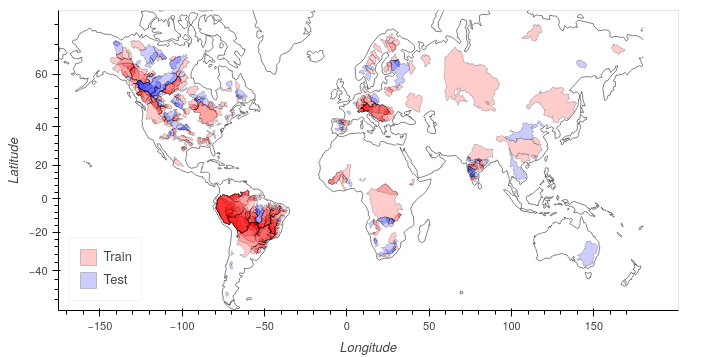
\includegraphics[width=\textwidth]{figure1}
\caption{Illustration of our dataset's catchment locations and split.catchment used for training and evaluating the correction model are shown in red and blue respectively.}
\end{figure}





For each river discharge measurement, we use the MERIT \ref{TOTO} topography to obtain the associated contributing basin. The water budget analysis performed at the basin scale uses the quantities of Table~\ref{table1} averaged over the basins.

Ideally, we would like that the basins cover all the environmental types; all the latitudes; small and large basins; tropical, temperate and polar weather; etc. However, we are truly limited here on the available river discharge stations. 

\subsection{Auxiliary variables}
\label{auxiliary_info}
We consider here a list of variables that are linked to the evaporation, at the large scale. 
We hope that these environmental information would be related to the errors of the evaporation estimates because if so, using them as inputs to a correction model could help us correct these errors. 
It is expected that errors in the satellite retrievals are conditioned on it.  
Several Environmental Indices (EI) have been retained : P − E, surface temperature, LAI (Leaf Area Index), SM (Soil Moisture), 
surface temperature from the ERA5 land operational archive, NDVI and EVI from MODIS [CIT]


Table~\ref{table1} provides in its bottom part the list of auxiliary variables that have been considered in this study.

%\begin{table}[h]
%\centering
%\begin{scriptsize}
%\begin{tabular} {l c c c c}
%\hline
%Variables & Coverage &  S. res. ($^\circ$)&  T. res.  & Reference \\
%\caption{Overview of the datasets used as inputs of the corection model. }
%\label{table2}
%\end{table}

%%%%%%%%%%%%%%%%%%%%%%%%%%%%%%%%%%%%%%%%%%%%%
\section{Analysis of the current evaporation datasets}
%%%%%%%%%%%%%%%%%%%%%%%%%%%%%%%%%%%%%%%%%%%%%

\subsection{Non closure of the water budget}
A first diagnostic to control the quality of the current evaporation datasets is to investigate how well the water cycle budget closes when we use the best available information for each water component. 
Montrer que cela ne ferme pas.

%\begin{wrapfigure}%{r}[0pt]{0.5\textwidth}%
\begin{figure}[h]
\centering
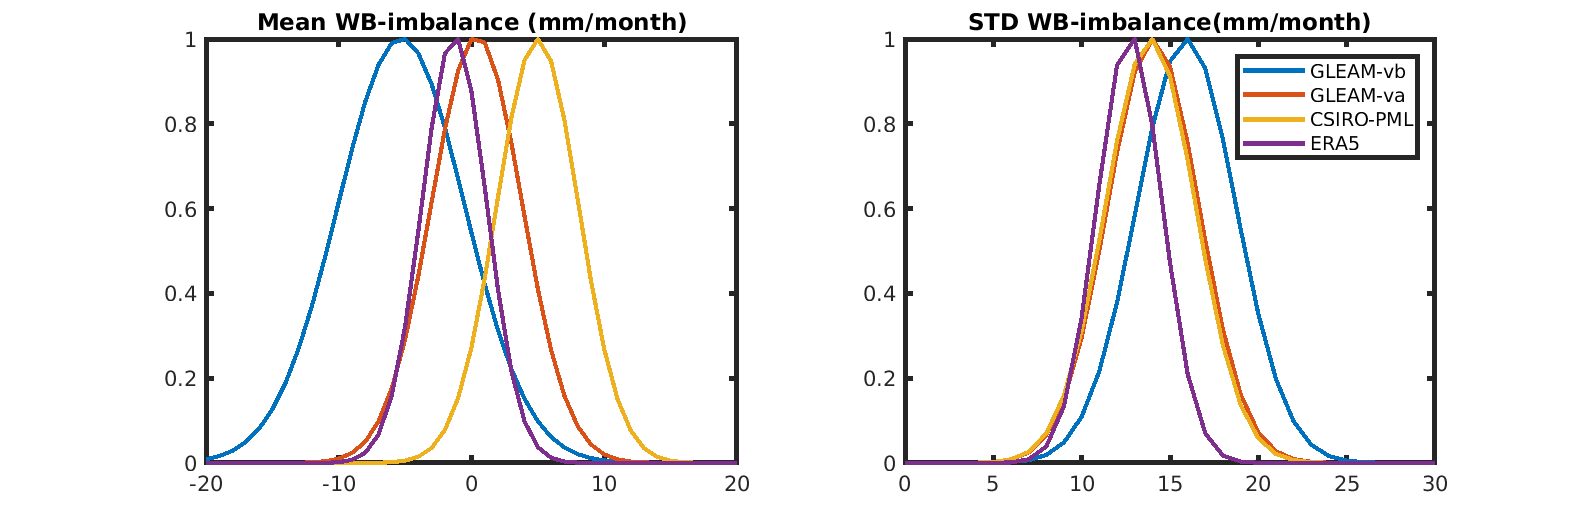
\includegraphics[width=\textwidth]{m_std_imb}
\caption{PDFs of the mean (left) and the STD (right) of the WB imbalance at catchment scale using the four ET datasets}
\end{figure}

This imbalance can result from errors in the $E$ estimate or it can result from problems in the three other datasets. 
In this study, we chose to use the best information on $P$, $dS$ and $R$ and then optimize $E$ because: 
(1) $P$ is a satellite observation that has been largely calibrated towards a network of {\it in situ} gauge measurements; 
(2) $dS$ is a variable at low temporal and spatial scale, measured by a unique satellite GRACE, that cannot easily be optimized, 
and (3) $R$ is a truly {\it in situ} measurement that is not perfect but we expect that it gives the right ranges of values for a particular river. 
Other strategies could be explored and they will be presented in the perspectives. 

\subsection{Optimal Interpolation (OI)}
To reduce the non-closure of the water cycle, the OI technique has been proposed to merge, in a coherent way, the various datasets presented in Section~\ref{dataset_integration}. 
The notations are presented in this section but more methodological details can be found in \cite{Aires2014a},. 
The last version of the integration methodology is well described in \cite{Pellet2019a}. 

The first step of the integration process consists in the "Simple Weighting" estimate that describes each water component based on all the available datasets \cite{Aires2014}. 
For each water component, all the datasets are first seasonally bias corrected to the ensemble mean climatology to avoid perturbation due to missing dataset over the period. 
The corrected datasets are then averaged. We denote $X_{SW} = (P_{SW}, E_{SW}, D_{SW}, \Delta S_{SW})$ where $SW$ stands for ``Simple weighting" the results of the merging.

It is then possible to write the conservation of water mass at the basin scale as a constraint applied on the state vector $X = (P, E, D, \Delta S)$. 
The WC budget constraint is expressed in Eq.~\ref{eq_closure3}. 
The problem can be written in the following way:

\begin{eqnarray}
\label{eq_closure3}
    & X^t               & = (P,\ E,\ R,\ \Delta S) \nonumber   \\
    & G                 &  = [1,\ -1,\ -1,\ -1]                             \\
    & X^t \cdot G^t &= 0, \nonumber
\end{eqnarray}
where $~^t$ is the transpose sign and $G$ the closure operator. 
The optimized solution of this problem can be expressed as a post-processing to impose the closure constrain on the previously obtained solution $X_{SW}$:
\begin{eqnarray}Figure 1 illustrates the location of training and test catchments for which we have gathered data. 
We investigate four different global ET datasets, 
for each of which we learn and evaluate corrections. 
Each dataset estimates ET using different methodology and thus showcase different error patterns. 
\label{eq_sol_pf}
     X_{PF} = (I - K_{PF} \cdot G) \cdot X_{SW}, 
\end{eqnarray}
where $K = B \cdot G^t (G \cdot B \cdot G^t )$, $PF$ stands for the ``Post-Filtering" of the previous solution $X_{SW}$, and $B$ is the {\it a priori} error covariance matrix of $X_{SW}$ that is specified here as :
\begin{eqnarray}
\label{eq_B}
B=\begin{pmatrix}
   \frac{5}{100}\bar{P}  &  0  &  0  &  0 \\
   0  &  \frac{10}{100}\bar{E} &  0  &  0 \\
   0  &  0  &  \frac{10}{100} \bar{\Delta S}  &  0 \\
   0  &  0  &  0  &  \frac{4}{100} \bar{R} \\
\end{pmatrix}.
\end{eqnarray}

The {\it a priori} specification of the uncertainties for $X_{SW}$ are derived from \cite{Dorigo2021} in which the authors reviewed carefully the literature on this topic.
This methodology allows obtaining a solution that closes the WC budget at the basin scale.

Advantages of the OI solution are numerous. 
It is a well established approach, with clear mathematical background. 
The sources of uncertainty are controlled in the input information, they are exploited to obtain the optimal solution, and an {\it a posteriori} uncertainty assessment is provided too. 
Each assumption is clear, and other physical or statistical constraints could be introduced in this framework. 

However, this method can be used only if the four water components ($P$, $E$, $dS$ and $R$) are available. 
This means that it can be used only on the basins presented in Section~\ref{def_basins}. 
An extrapolation strategy would be required in order to obtain results at the global scale. 
This has been attempted for instance in \ref{TOTO}. 
Another inconvenient is that the integration is performed at the basin scale and 
we would like to obtain results at the original spatial resolution of the satellite datasets (the pixel scale) instead.

\subsection{Closure Error Decomposition}

The objective of our correction model is to transform the $E$ estimate into an $\hat E$ that is closer to the optimal interpolation solution $E_{OI}$. To measure the improvements, it is therefore useful to monitor the sum of squares of the errors $\Delta = \hat E - E_{OI}$ between these two quantities, for each location $i$.
This sum of square errors can be decomposed into three terms:
\begin{equation}
\sum_{t=1}^T {\Delta(i,t)}^2 =  \left(Bias\left(\Delta_i  \right) \right)^2 + Var\left( \Delta_{seas} \right) + Var\left( \Delta_{an} \right)
\end{equation}

The first term in the right hand part of the equation is the total Mean Square Error (MSE), for each location. 
It can be decomposed in three terms: squared bias, seasonal variance (subscript $_{seas}$) and variance of anomalies to the season (subscript $_{an}$).
 Squared bias represents the overall constant error while seasonal variance weights the capacity to reconstruct the season of $E_{OI}$ from the model. 
Finally the variance of anomalies penalize the reconstruction of the seasonal anomalies. 
From these three terms is it possible to investigate which kind of error the model reduce better.

%%%%%%%%%%%%%%%%%%%%%%%%%%%%%%%%%%%%%%%%%%%%%
\section{A correction model}
%%%%%%%%%%%%%%%%%%%%%%%%%%%%%%%%%%%%%%%%%%%%%

\subsection{A correction model strategy}

The strategy proposed here is based on the OI results obtained on the set of basins around the world (Section~\ref{def_basins}). 
The objective is to set up a statistical model that would be trained with the OI results and that could be applied at the global scale, at the pixel resolution. 
Such a model should benefit from auxiliary information of Section~\ref{auxiliary_info} to help the model extrapolating results to similar environments encountered in the training database of the basins. 
The auxiliary information should also be related to the satellite dataset errors so that the model can use them to attempt correcting them.
 We should find a way too to train the model with basin-scale data (from the OI) but be able to apply it at the pixel scale. 
This is not a straightforward task as states might differ at the two spatial resolution.

\subsection{A probabilistic formulation}

Our goal is to find a function $f_{\theta}(x)$ that regresses pixel-wise ET corrections $y$ of monthly ET values $E$ from inputs $x$.
We refer to the true, correct evaporation values as $\hat E = E + y$.
Note that we do not have knowledge of these correct pixelwise evaporation values $\hat E$.
Instead, we have access to estimations of their sum over hydrological catchments using the OI methodology described in the previous section.

We thus take a probabilistic view on the ET estimates $E$ provided by global datasets, and the corrections $y$ we aim to provide.
We consider each dataset to provide us with prior knowledge on the pixel-wise ET $\hat E$ 
in the form of a Gaussian distribution centered on $E$:  $P(\hat E)=\mathcal{N}(E | \sigma_E)$. 
A recent review paper \cite{XXX} has estimated the relative uncertainty of current global ET datasets around 7\%.
Following their estimation, we thus parameterize the prior with $\sigma_E= \frac{7 \cdot E}{100}$.
We can rewrite this prior distribution in terms of $y$ as $P(y)=\mathcal{N}(0 | \sigma_E)$.

Similarly, we explicitly model uncertainty over the corrections $y$ estimated from inputs $x$ by defining a conditional distribution $p(y|x)$.
Following Bayesian terminology, we refer to this conditional distribution as the likelyhood and parameterize it as the Gaussian distribution $p(y|x)=\mathcal{N}(h_\theta(x) | \sigma_y)$
The paramerized function $h_\theta(x)$ provides the mean of the likelyhood.
We estimate the parameters $\theta$ by fitting $h_\theta(x)$ to the training data, 
as explained in the following subsection.
$\sigma_{y}$ quantifies the uncertainty over the regressed corrections.
We use a constant uncertainty estimat $\sigma_{y}$ over all spatiotemporal datapoints,
whose value we calibrate on a held-out validation split.

Given the prior distribution $P(y)$ provided by global ET datasets and the likelihood $p(y|x)$ derived from inputs $x$,
we define the correction model $f_\theta(x)$ as the Maximum A Posteriori (MAP), i.e.; 
the maximum over the posterior distribution:

\begin{flalign}
f_{\theta}(x)=max_{y} p(y | x)P(y) \\
f_{\theta}(x)=max_{y} \mathcal{N}(h_\theta(x) | \sigma_y) \times \mathcal{N}(0 | \sigma_E)
\end{flalign}

As both distributions are considered Gaussian, we can derive a closed-form formulation for $f_\theta(x)$ as:

\begin{flalign}
f_{\theta}(x)= \frac{\sigma_E^2 \times h_{\theta}(x) + 0 \times \sigma_y^2}{\sigma_y^2 + \sigma_E^2} \\
f_{\theta}(x)= \frac{h_{\theta}(x)}{1 + \frac{100 \times \sigma_y^2}{7 \times E}}
\end{flalign}

The rationale for this MAP formulation is that it allows to scale the correction with gloabel ET dataset estimates.
Indeed, we expect ET estimates to be less error-prone (in absolute values) in arid situations 
where ET is close to zero than in humid situations where ET estimates take large values.
In section XXX, we conduct an ablation study to illustrate the impact of this MAP formulation and contrast 
our approach to the more straightforward maximum-likelihood correction estimates.

\subsection{Catchement-level supervision}

Although $f_\theta(x)$ regresses ET corrections at the pixel level, 
ground-truth pixel-wise corrections $y$ are not available to supervise the model training.
Instead, the OI methodology described in Section XXX provides us with catchment-level ET corrections $y$
representing the sum of pixel-wise ET corrections over each catchment area.

Different strategies can be considered to regress pixel-level corrections from catchment-level ground truth.
Maybe the most straightforward approach would be to aggregate inputs $x$ at the catchment level so as
to train the model on catchment-level input-output associations, 
and to generalize the learned associations to pixel-level data.
Unfortunately, we found this approach to yield sub-optimal corrections.
We conjecture that this is due to the fact that the input features distribution 
at the pixel-level and at the catchment-level differ significantly due 
to the smoothing effect of aggregating input features with possibly high 
intra-catchment variance over large catchment areas.

Instead, we adopt a different strategy, in which we first apply the model on the pixels of each catchments, 
yielding a set of pixel-wise corrections for a given catchment.
We then aggregate the model output by summation, and regress the aggregated sum of corrections to the catchment label $y$. 
For a given catchment $c$ and month $t$, the catchment-level correction $F_{\theta}(c, t)$ computed by our model is thus:

\begin{flalign}
F_{\theta}(c, t)=\sum_{x \in X(c,t)} f_{\theta}(x)
\end{flalign}

Using a Mean Squared Error (MSE) loss, 
we define our supervision signal $\mathcal{L}$ and optimization problem as:

\begin{flalign}
e_\theta(c,t) = F_{\theta}(c,t) - y(c,t) \\
\mathcal{L(\theta)}=\frac{1}{T}\sum_{c \in C} \sum_{t \in T}  e_\theta(c,t) \\
\theta* = min_{\theta \in \Theta}\mathcal{L(\theta)}
\end{flalign}

In Section XXX, we conduct an ablation study to demonstrate the benefit of using this problem definition 
over other strategies including the input aggregation scheme described above.

\subsection{Experiment details}

Following standard ML methodology, we split our dataset into a training and validation set, 
on which we respectively train and calibrate the model,
and a test set we use to evaluate the ability of the model to generalize its learned corrections to unseen data.
We split our dataset catchment-wise so as to evaluate the model ability to generalize to unseen locations.
The splits were defined so that every overlapping catchments belong to the same split 
so as to avoid data leak from the training to the test set.
Larger catchments have been shown to XXX. 
We have thus included all the largest catchments, those with a drainage area superior to XXX squared killometers, 
to the training set so as to ensure that the model is trained to regress corrections with the least uncertainty.
Figure XXX illustrates the resulting training and test splits. 
We used a set of XXX randomly selected catchments from the training set as validation 
data to control for both overfitting by early stopping and to calibrate the uncertainty parameter $\sigma_y$.

The function $h_\theta$ was parameterized as a Multi-Layer Perceptron (MLP) with four hidden layers.
Each hidden layer consists of 512 neurons with Rectified Linear Unit (ReLU) activations.
We apply a scaled hyperbolic tangent at the output of the model as a soft thresholding strategy 
to bound the model output between two sigmas of the training split ground-truth corrections.
This strategy is used as a safe-guard to prevent rare extremes in the input distribution from 
generating physically meaningless ET correction outliers.
  
The model wieghts were initialized using the He initialization scheme \cite{XXX}.
The model was trained to minimize the loss function (Equation XXX) 
using the Adam optimizer, with a learning rate of $0.001$.
We used default $\beta$ parameter values of $(.5, .99)$.
For memory constraint, we used a mini-batch sampling strategy in which each batch consists of
XXX catchments randomly sampled from the dataset. 
For each selected catchment, every XXX month.
We trained the model for XXX epochs.
Our implementation is based on the PyTorch framework \cite{XXX}, and ran on XXX Nvidia GPUs. 

%\begin{wrapfigure}%{r}[0pt]{0.5\textwidth}%
\begin{figure}[h]
%\centering
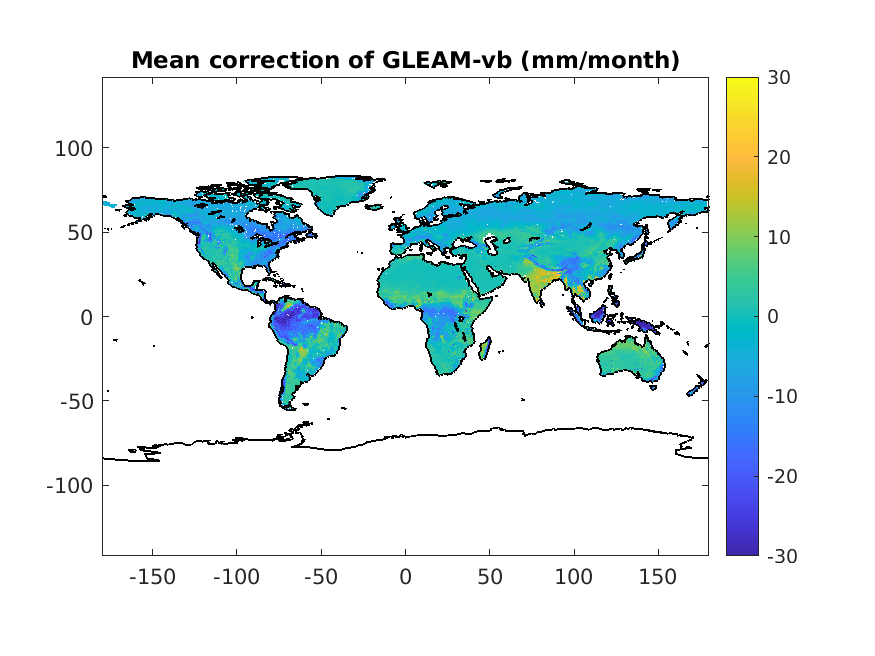
\includegraphics[width=0.6\textwidth]{patchm1}
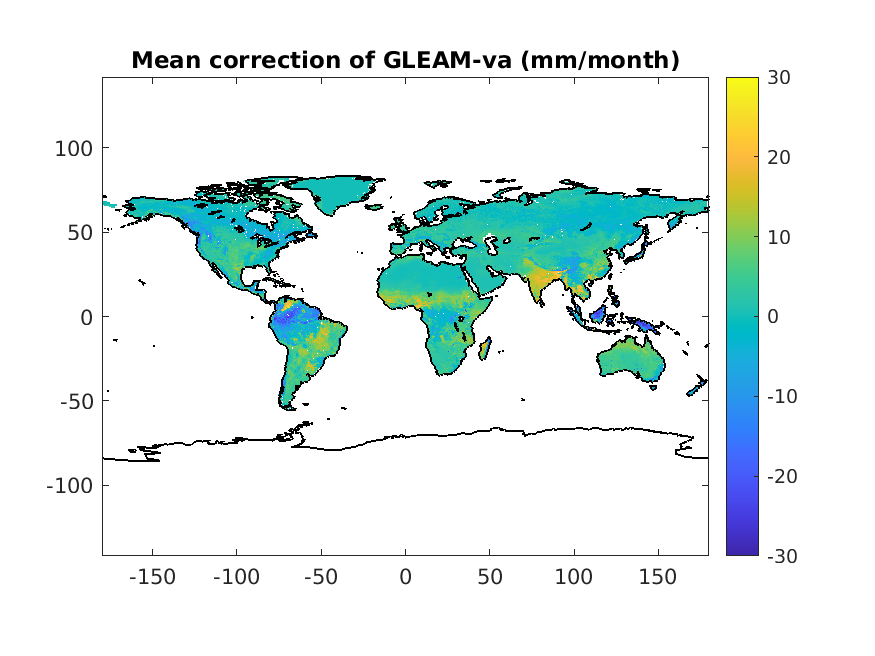
\includegraphics[width=0.6\textwidth]{patchm2}
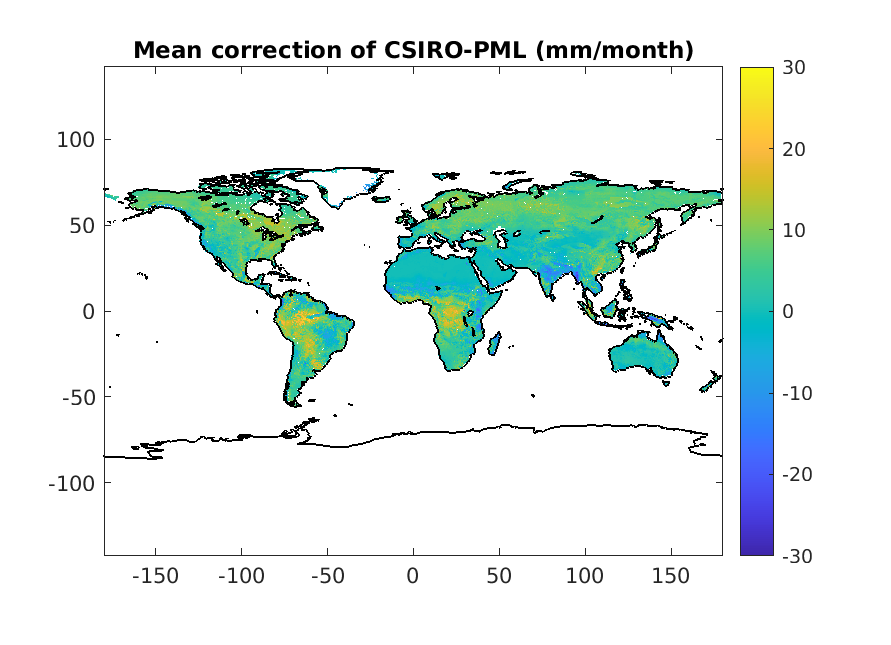
\includegraphics[width=0.6\textwidth]{patchm3}
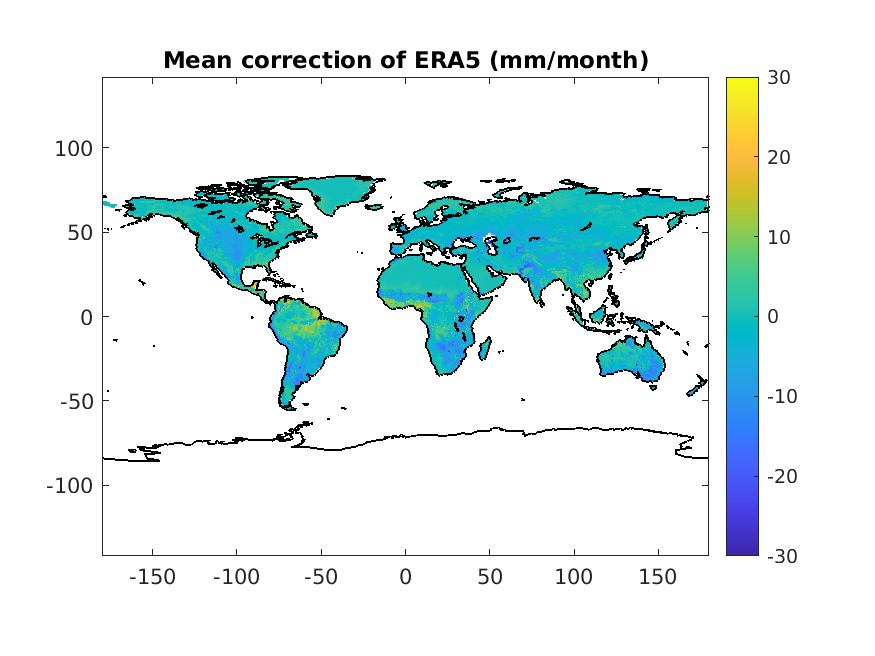
\includegraphics[width=0.6\textwidth]{patchm4}
\caption{Mean ML-based correction patch for the ET datasets}
\end{figure}

%%%%%%%%%%%%%%%%%%%%%%%%%%%%%%%%%%%%%%%%%%%%%
\section{Evaluation}
%%%%%%%%%%%%%%%%%%%%%%%%%%%%%%%%%%%%%%%%%%%%%

Through experiments, we aim to XXX.

\subsection{Water Cycle Closure Results}

\begin{table}[h]
\centering
\begin{scriptsize}
\begin{tabular} {l c c c c}
\hline
Dataset & Org. &   Org. + patch static &  Org.+ patch Seas. &  Org.+ patch monthly \\
\hline 
GLEAM vb &  14.5   &   13.1    &  10.9    &  9.9   \\
GLEAM va &  13.6   &   12.1    &  11.1    &  10.1  \\
CSIRO    &  14.8   &   13.4    &  11.7    &  10.1  \\
ERA-5    &  12.6   &   12.0    &  11.1    &  10.0  \\
\hline
\end{tabular}
\end{scriptsize}
\caption{WB imbalance reduction using patch with various temporal resolution: static, seasonal and monthly correction. }
\label{table1}
\end{table}

\subsection{Validation using flux tower evaporation data}

\begin{figure}[h]
\centering
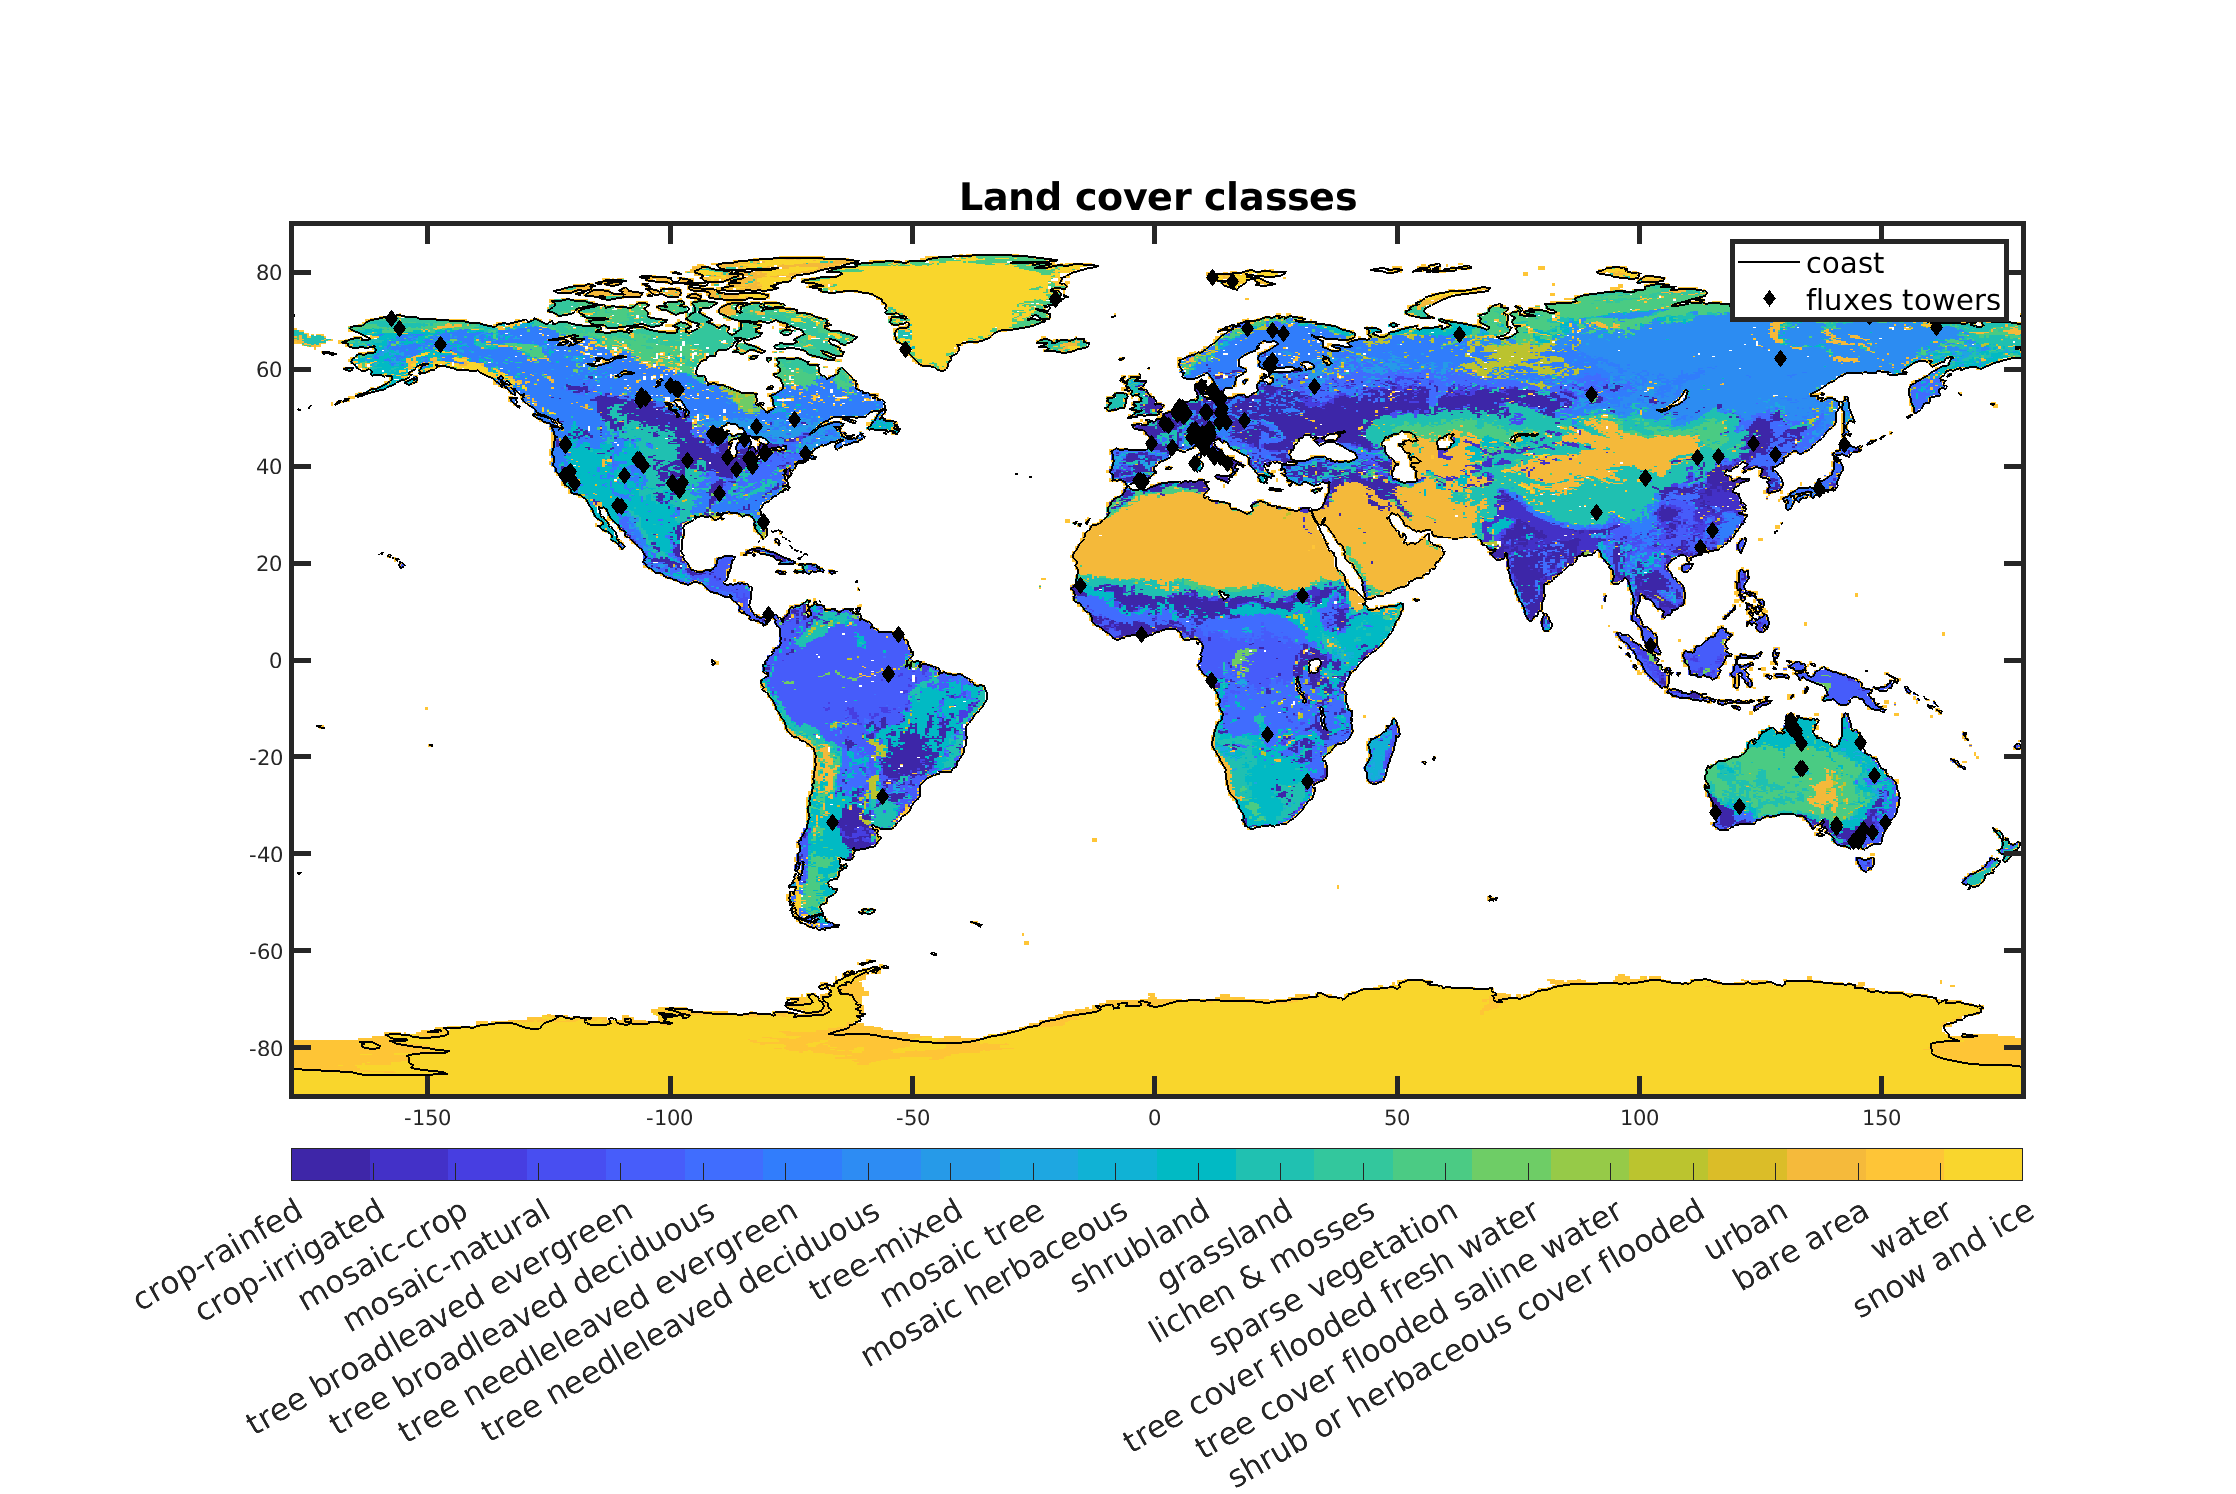
\includegraphics[width=0.9\textwidth]{LCC_025.png}
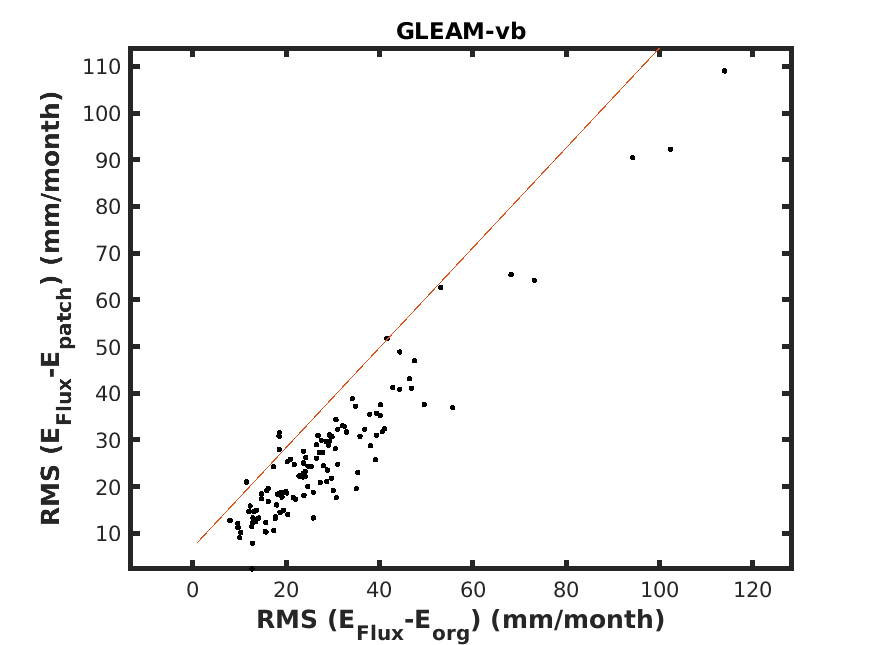
\includegraphics[width=0.24\textwidth]{squatter_rmse1.png}
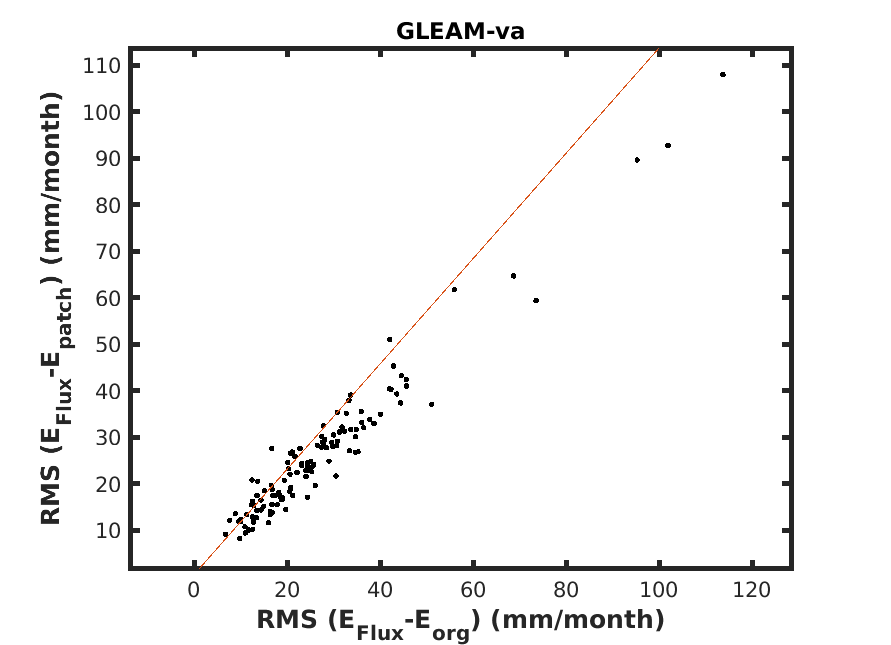
\includegraphics[width=0.24\textwidth]{squatter_rmse2.png}
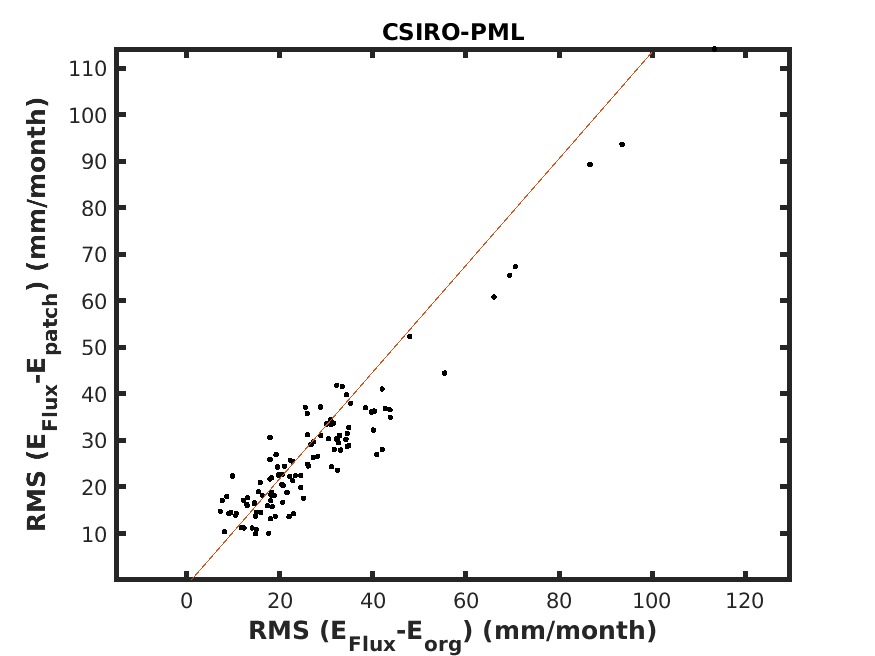
\includegraphics[width=0.24\textwidth]{squatter_rmse3.png}
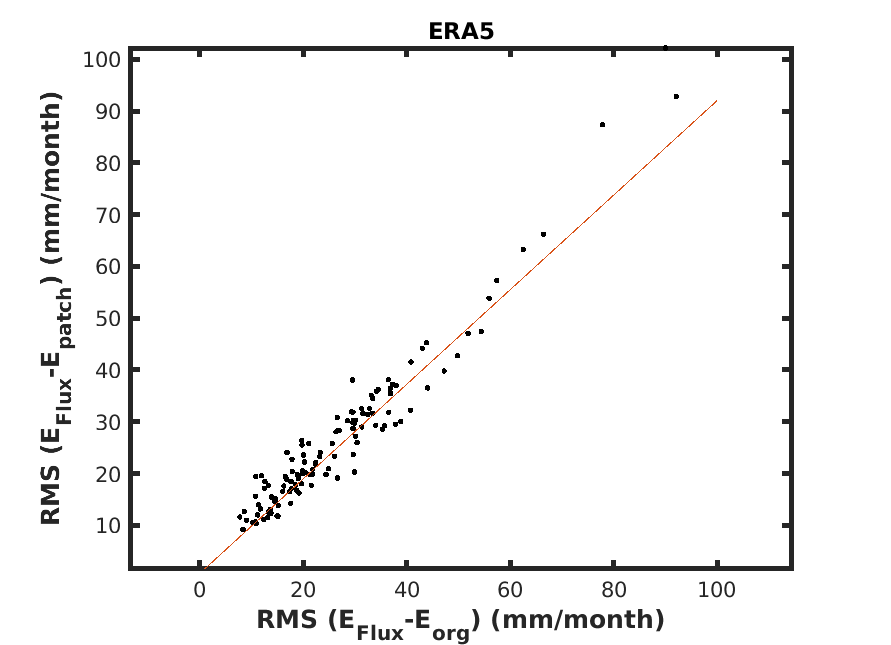
\includegraphics[width=0.24\textwidth]{squatter_rmse4.png}
\caption{Top : location of the {\it in situ} fluxes tower used in the evaluation and the main land cover class at 0.25$^\cir$ resolution. Bottom: scatter plot of the ET difference between {\it in situ} and satellite ET before (xaxis) and after (yaxis) correction. The 1:1 line is indicated in red.}
\end{figure}


\begin{table}[h]
\centering
\begin{scriptsize}
\begin{tabular} {l c c c c}
\hline
Dataset & Org. &   Org. + patch static &  Org.+ patch Seas. &  Org.+ patch monthly \\
\hline 
 GLEAM vb &   28.4 &  27.2  & 26.4  & 26.7\\
 GLEAM va &  27.2  & 26.8 &  26.5  & 26.7\\
 CSIRO-PML &  27.8  & 27.5  & 28.0  & 28.0\\
 ERA-5 & 27.4  & 27.1  & 27.2  & 27.2\\
\hline 
\end{tabular}
\end{scriptsize}
\caption{Evaluation using {\it in situ} Flux tower from fluxnet.}
\label{table1}
\end{table}

% GLEAM vb &    0.73 &    0.73  &    0.74 &   0.74 \\
%GLEAM va &     0.74 &    0.74 &    0.7432 &   0.74 \\
%  CSIRO-PML &    0.75 &    0.75 &    0.73 &    0.73 \\
% ERA5 &  0.72 &    0.72 &    0.71 &    0.72

\subsection{land cover results}


\begin{figure}[h]
%\centering
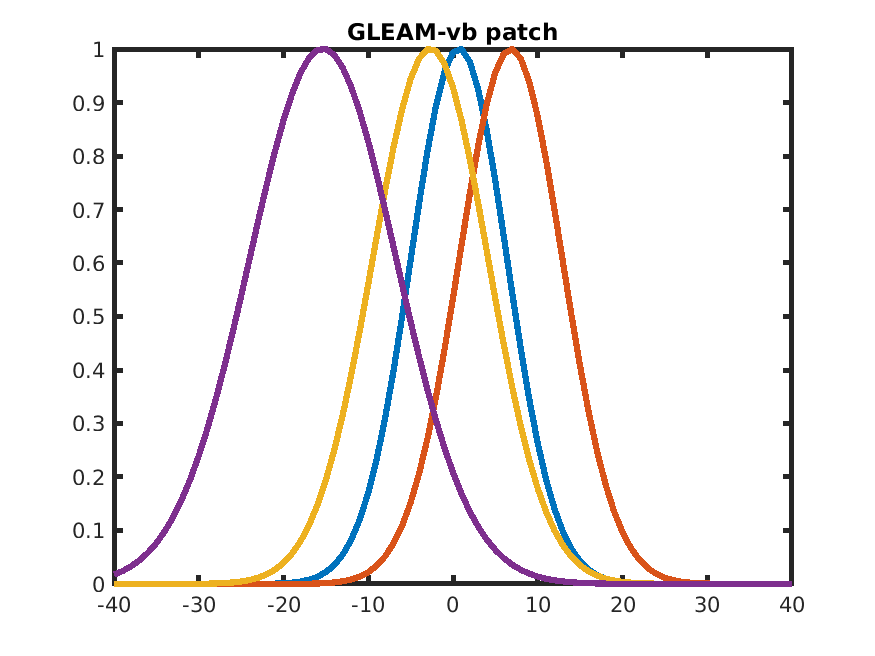
\includegraphics[width=0.5\textwidth]{lcc_patch_1.png}
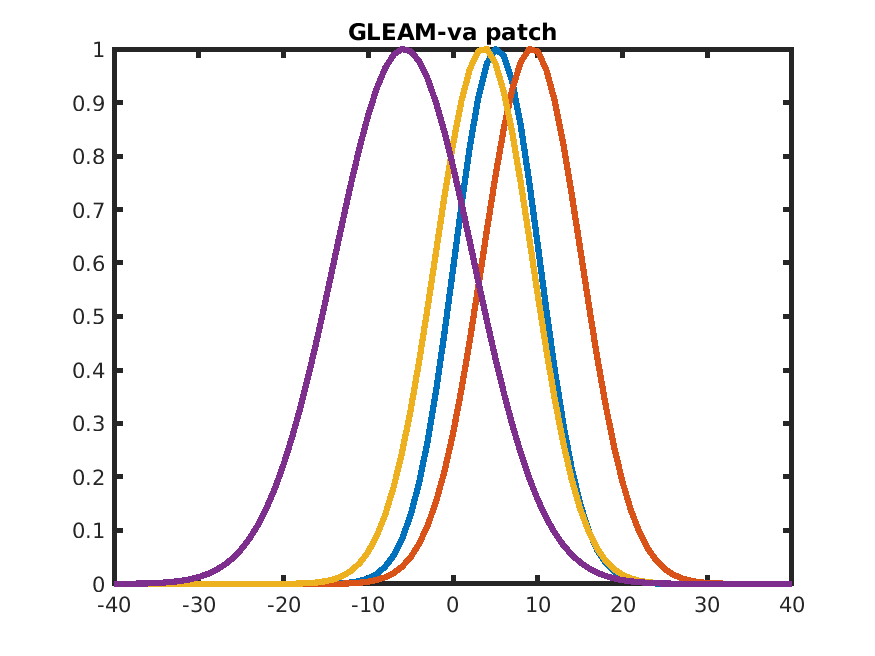
\includegraphics[width=0.5\textwidth]{lcc_patch_2.png}
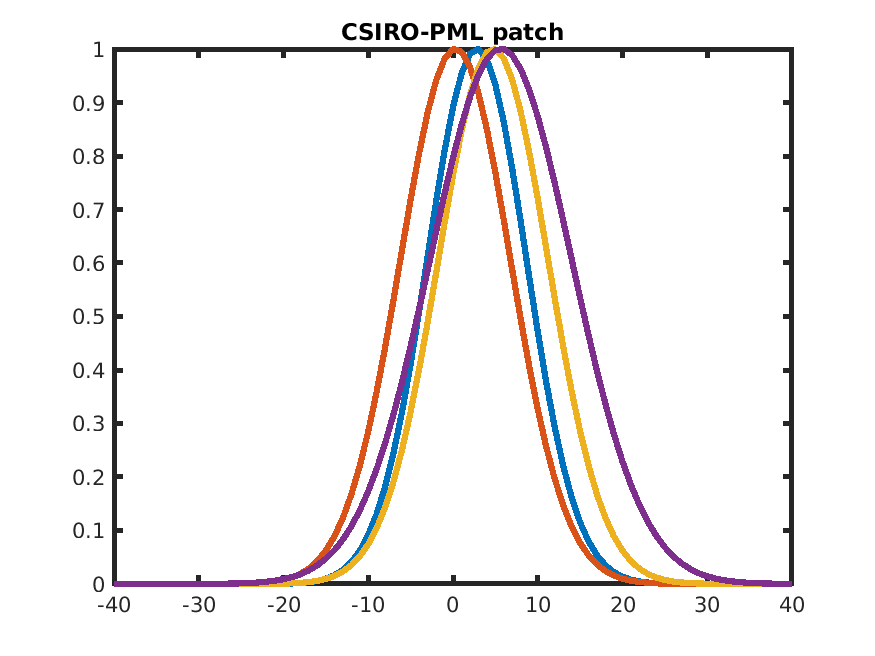
\includegraphics[width=0.5\textwidth]{lcc_patch_3.png}
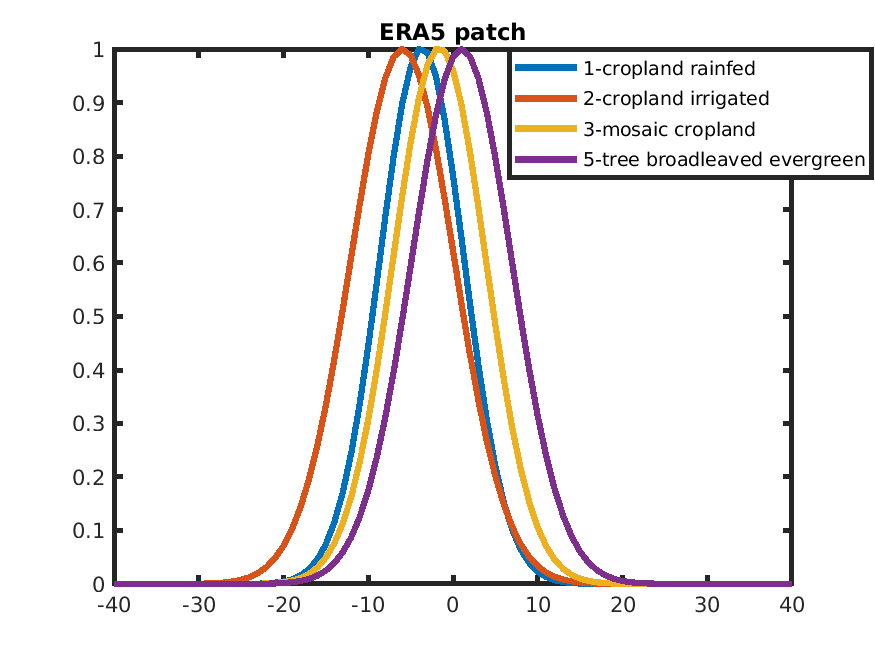
\includegraphics[width=0.5\textwidth]{lcc_patch_4.png}
\caption{Mean correction of the four ET datasets for various land cover classes}
\end{figure}


\subsection{quality flag}

carte dispersion
identifier dispersion comme problem 

\begin{figure}[h]
%\centering
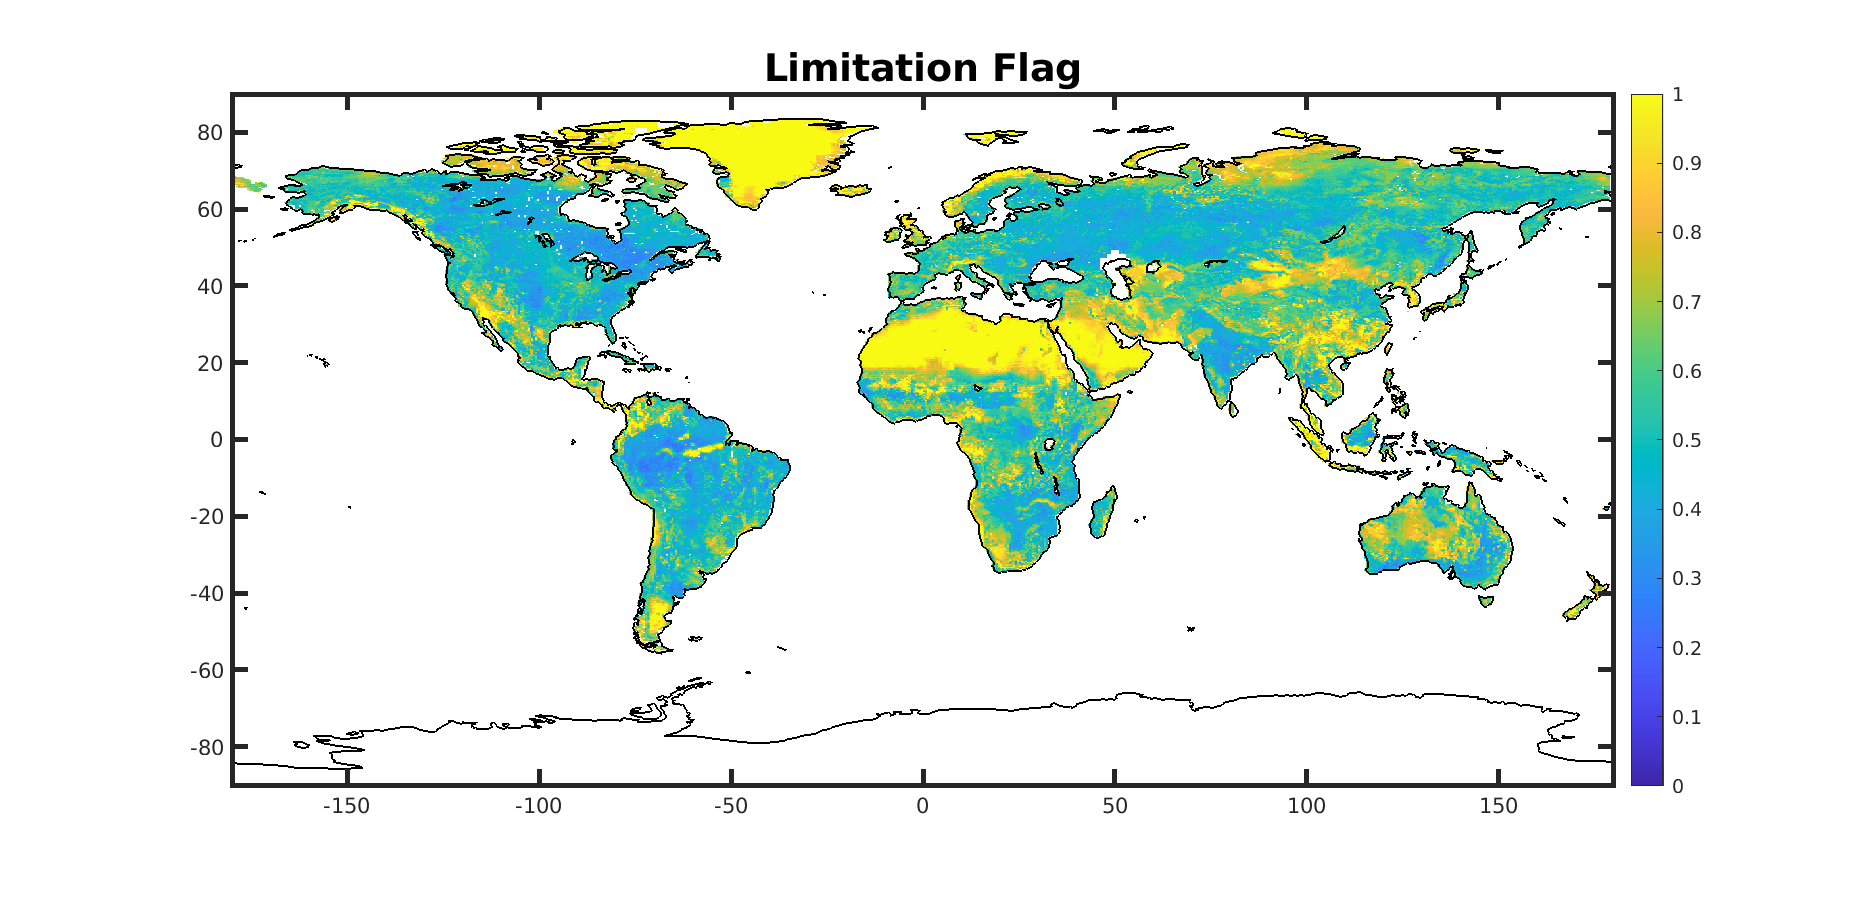
\includegraphics[width=\textwidth]{std_flag.png}
\caption{Error flag (1 is problematic region)}
\end{figure}


\subsection{reconstructed river discharge measurements compared CAma } 
%\subsection{A new E reference (2000-2015)}
\subsubsection{over miss}






%%%%%%%%%%%%%%%%%%%%%%%%%%%%%%%%%%%%%%%%%%%%%
\section{Conclusions and perspectives}
%%%%%%%%%%%%%%%%%%%%%%%%%%%%%%%%%%%%%%%%%%%%%
Optimal interpolation is the right framework to optimize evaporation estimates: it uses observations on the other water components and the water budget closure, to obtain an indirect constrain on the evaporation. Each source of information is weighted by its uncertainty specifications. However, optimal interpolation can only be used at the basin level and for basins where river discharge measurements are available. A new artificial intelligence based model was proposed here to learn from the OI on these basins, and obtain an evaporation correction model applicable at the pixel level and at the global scale. 

The model proposed here can be 

Exemple d'un modele qui est entrainé sur des gros bassins, et qu'on peut appliqué sur du pixelaire. On devrait pouvoir utiliser cette strategie pour faire du downscaling.

Faire l'optimization de toutes les composantes (Matt) en utilisant un meme NN.









%\section{= enter section title =}
%Text here ===>>>


%%

%  Numbered lines in equations:
%  To add line numbers to lines in equations,
%  \begin{linenomath*}
%  \begin{equation}
%  \end{equation}
%  \end{linenomath*}



%% Enter Figures and Tables near as possible to where they are first mentioned:
%
% DO NOT USE \psfrag or \subfigure commands.
%
% Figure captions go below the figure.
% Table titles go above tables;  other caption information
%  should be placed in last line of the table, using
% \multicolumn2l{$^a$ This is a table note.}
%
%----------------
% EXAMPLE FIGURES
%
% \begin{figure}
% \includegraphics{example.png}
% \caption{caption}
% \end{figure}
%
% Giving latex a width will help it to scale the figure properly. A simple trick is to use \textwidth. Try this if large figures run off the side of the page.
% \begin{figure}
% \noindent\includegraphics[width=\textwidth]{anothersample.png}
%\caption{caption}
%\label{pngfiguresample}
%\end{figure}
%
%
% If you get an error about an unknown bounding box, try specifying the width and height of the figure with the natwidth and natheight options. This is common when trying to add a PDF figure without pdflatex.
% \begin{figure}
% \noindent\includegraphics[natwidth=800px,natheight=600px]{samplefigure.pdf}
%\caption{caption}
%\label{pdffiguresample}
%\end{figure}
%
%
% PDFLatex does not seem to be able to process EPS figures. You may want to try the epstopdf package.
%

%
% ---------------
% EXAMPLE TABLE
% Please do NOT include vertical lines in tables
% if the paper is accepted, Wiley will replace vertical lines with white space
% the CLS file modifies table padding and vertical lines may not display well
%

%% SIDEWAYS FIGURE and TABLE
% AGU prefers the use of {sidewaystable} over {landscapetable} as it causes fewer problems.
%
% \begin{sidewaysfigure}
% \includegraphics[width=20pc]{figsamp}
% \caption{caption here}
% \label{newfig}
% \end{sidewaysfigure}
%
%  \begin{sidewaystable}
%  \caption{Caption here}
% \label{tab:signif_gap_clos}
%  \begin{tabular}{ccc}
% one&two&three\\
% four&five&six
%  \end{tabular}
%  \end{sidewaystable}

%% If using numbered lines, please surround equations with \begin{linenomath*}...\end{linenomath*}
%\begin{linenomath*}
%\begin{equation}
%y|{f} \sim g(m, \sigma),
%\end{equation}
%\end{linenomath*}

%%% End of body of article

%%%%%%%%%%%%%%%%%%%%%%%%%%%%%%%%
%% Optional Appendix goes here
%
% The \appendix command resets counters and redefines section heads
%
% After typing \appendix
%
%\section{Here Is Appendix Title}
% will show
% A: Here Is Appendix Title
%
%\appendix
%\section{Here is a sample appendix}

%%%%%%%%%%%%%%%%%%%%%%%%%%%%%%%%%%%%%%%%%%%%%%%%%%%%%%%%%%%%%%%%
%
% Optional Glossary, Notation or Acronym section goes here:
%
%%%%%%%%%%%%%%
% Glossary is only allowed in Reviews of Geophysics
%  \begin{glossary}
%  \term{Term}
%   Term Definition here
%  \term{Term}
%   Term Definition here
%  \term{Term}
%   Term Definition here
%  \end{glossary}

%
%%%%%%%%%%%%%%
% Acronyms
%   \begin{acronyms}
%   \acro{Acronym}
%   Definition here
%   \acro{EMOS}
%   Ensemble model output statistics
%   \acro{ECMWF}
%   Centre for Medium-Range Weather Forecasts
%   \end{acronyms}

%
%%%%%%%%%%%%%%
% Notation
%   \begin{notation}
%   \notation{$a+b$} Notation Definition here
%   \notation{$e=mc^2$}
%   Equation in German-born physicist Albert Einstein's theory of special
%  relativity that showed that the increased relativistic mass ($m$) of a
%  body comes from the energy of motion of the body—that is, its kinetic
%  energy ($E$)—divided by the speed of light squared ($c^2$).
%   \end{notation}


%%%%%%%%%%%%%%%%%%%%%%%%%%%%%%%%%%%%%%%%%%%%%%%

\acknowledgments
This section is optional. Include any Acknowledgments here.
The acknowledgments should list:\\
All funding sources related to this work from all authors\\
Any real or perceived financial conflicts of interests for any author\\
Other affiliations for any author that may be perceived as having a conflict of interest with respect to the results of this paper.\\
It is also the appropriate place to thank colleagues and other contributors. AGU does not normally allow dedications.


%% ------------------------------------------------------------------------ %%
%% References and Citations

%%%%%%%%%%%%%%%%%%%%%%%%%%%%%%%%%%%%%%%%%%%%%%%
%
% \bibliography{<name of your .bib file>} don't specify the file extension
%
% don't specify bibliographystyle

% In the References section, cite the data/software described in the Availability Statement (this includes primary and processed data used for your research). For details on data/software citation as well as examples, see the Data & Software Citation section of the Data & Software for Authors guidance
% https://www.agu.org/Publish-with-AGU/Publish/Author-Resources/Data-and-Software-for-Authors#citation

%%%%%%%%%%%%%%%%%%%%%%%%%%%%%%%%%%%%%%%%%%%%%%%
%\bibliographystyle{ametsoc2014}
\bibliography{library}



%Reference citation instructions and examples:
%
% Please use ONLY \cite and \citeA for reference citations.
% \cite for parenthetical references
% ...as shown in recent studies (Simpson et al., 2019)
% \citeA for in-text citations
% ...Simpson et al. (2019) have shown...
%
%
%...as shown by \citeA{jskilby}.
%...as shown by \citeA{lewin76}, \citeA{carson86}, \citeA{bartoldy02}, and \citeA{rinaldi03}.
%...has been shown \cite{jskilbye}.
%...has been shown \cite{lewin76,carson86,bartoldy02,rinaldi03}.
%... \cite <i.e.>[]{lewin76,carson86,bartoldy02,rinaldi03}.
%...has been shown by \cite <e.g.,>[and others]{lewin76}.
%
% apacite uses < > for prenotes and [ ] for postnotes
% DO NOT use other cite commands (e.g., \citet, \citep, \citeyear, \citealp, etc.).
% \nocite is okay to use to add references from your Supporting Information
%



\end{document}



More Information and Advice:

%% ------------------------------------------------------------------------ %%
%
%  SECTION HEADS
%
%% ------------------------------------------------------------------------ %%

% Capitalize the first letter of each word (except for
% prepositions, conjunctions, and articles that are
% three or fewer letters).

% AGU follows standard outline style; therefore, there cannot be a section 1 without
% a section 2, or a section 2.3.1 without a section 2.3.2.
% Please make sure your section numbers are balanced.
% ---------------
% Level 1 head
%
% Use the \section{} command to identify level 1 heads;
% type the appropriate head wording between the curly
% brackets, as shown below.
%
%An example:
%\section{Level 1 Head: Introduction}
%
% ---------------
% Level 2 head
%
% Use the \subsection{} command to identify level 2 heads.
%An example:
%\subsection{Level 2 Head}
%
% ---------------
% Level 3 head
%
% Use the \subsubsection{} command to identify level 3 heads
%An example:
%\subsubsection{Level 3 Head}
%
%---------------
% Level 4 head
%
% Use the \subsubsubsection{} command to identify level 3 heads
% An example:
%\subsubsubsection{Level 4 Head} An example.
%
%% ------------------------------------------------------------------------ %%
%
%  IN-TEXT LISTS
%
%% ------------------------------------------------------------------------ %%
%
% Do not use bulleted lists; enumerated lists are okay.
% \begin{enumerate}
% \item
% \item
% \item
% \end{enumerate}
%
%% ------------------------------------------------------------------------ %%
%
%  EQUATIONS
%
%% ------------------------------------------------------------------------ %%

% Single-line equations are centered.
% Equation arrays will appear left-aligned.

Math coded inside display math mode \[ ...\]
 will not be numbered, e.g.,:
 \[ x^2=y^2 + z^2\]

 Math coded inside \begin{equation} and \end{equation} will
 be automatically numbered, e.g.,:
 \begin{equation}
 x^2=y^2 + z^2
 \end{equation}


% To create multiline equations, use the
% \begin{eqnarray} and \end{eqnarray} environment
% as demonstrated below.
\begin{eqnarray}
  x_{1} & = & (x - x_{0}) \cos \Theta \nonumber \\
        && + (y - y_{0}) \sin \Theta  \nonumber \\
  y_{1} & = & -(x - x_{0}) \sin \Theta \nonumber \\
        && + (y - y_{0}) \cos \Theta.
\end{eqnarray}

%If you don't want an equation number, use the star form:
%\begin{eqnarray*}...\end{eqnarray*}

% Break each line at a sign of operation
% (+, -, etc.) if possible, with the sign of operation
% on the new line.

% Indent second and subsequent lines to align with
% the first character following the equal sign on the
% first line.

% Use an \hspace{} command to insert horizontal space
% into your equation if necessary. Place an appropriate
% unit of measure between the curly braces, e.g.
% \hspace{1in}; you may have to experiment to achieve
% the correct amount of space.


%% ------------------------------------------------------------------------ %%
%
%  EQUATION NUMBERING: COUNTER
%
%% ------------------------------------------------------------------------ %%

% You may change equation numbering by resetting
% the equation counter or by explicitly numbering
% an equation.

% To explicitly number an equation, type \eqnum{}
% (with the desired number between the brackets)
% after the \begin{equation} or \begin{eqnarray}
% command.  The \eqnum{} command will affect only
% the equation it appears with; LaTeX will number
% any equations appearing later in the manuscript
% according to the equation counter.
%

% If you have a multiline equation that needs only
% one equation number, use a \nonumber command in
% front of the double backslashes (\\) as shown in
% the multiline equation above.

% If you are using line numbers, remember to surround
% equations with \begin{linenomath*}...\end{linenomath*}

%  To add line numbers to lines in equations:
%  \begin{linenomath*}
%  \begin{equation}
%  \end{equation}
%  \end{linenomath*}





